\section{Fallout3}

\begin{figure}[htbp]
\begin{center}
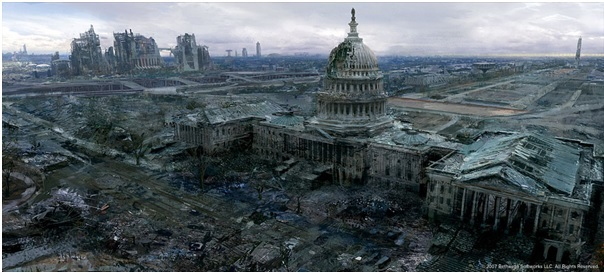
\includegraphics[width=.60\textwidth]{./imagenes/fallout3.jpg}
\caption{Fallout3}
\label{Fallout3}
\end{center}
\end{figure}
Fallout 3 tiene lugar en el año 2278, 200 años después de que una guerra mundial por los recursos culminara en un holocausto nuclear. La ambientación es una región post-apocalíptica y retrofuturista que abarca gran parte del estado de Washington D.C., el nordeste deVirginia y partes de Maryland. El entorno del juego incluye edificios de la vida real devastados por la guerra como la Casa Blanca, elMonumento a Jefferson, el Monumento a Lincoln, el Cementerio Nacional de Arlington y el Monumento a Washington. El área en el que el juego está ubicado, conocida como Yermo Capital (Capital Wasteland), cuenta con una serie de pequeños asentamientos donde los sobrevivientes de la Gran Guerra se hospedan. Muchos de los habitantes murieron durante el holocausto nuclear y el Yermo Capital es ahora poco más que una tierra árida casi desprovista de agua potable, comida, plantas y vida animal a causa de los niveles extremos de radiación. A pesar de esto existe un pequeño asentamiento en el norte del Yermo Capital donde la vida vegetal prevalece.


\subsubsection{¿Por qué es uno de mis juegos favoritos?}
\begin{itemize}
\item[José Salas] El juego comienza dentro del Refugio 101, donde ellos creen haber nacido originalmente, antes de aventurarse a las afueras del refugio donde se enfrentarán a la peligrosa verdad. Yermo Capital es hogar de criaturas mutadas como vacas de dos cabezas, escorpiones de proporciones colosales, así como de grupos de sobrevivientes hostiles como saqueadores o guerrilleros. En el área que comprende Washington en el Yermo Capital muchos de los caminos están bloqueados por pilas de ruinas y el jugador deberá utilizar los metros subterráneos que conectan la ciudad.

\end{itemize}